\appendix

\section{Pipeline and prompts}
\label{app:prompts}

\begin{figure*}[t]
\centering
\resizebox{\textwidth}{!}{% Figure 1: evidence pipeline (schematic; contains no numbers).
\begin{tikzpicture}[
  font=\footnotesize,
  box/.style={draw, rounded corners=2pt, align=center, minimum height=9mm, text width=19mm, fill=white},
  opt/.style={box, dashed},
  exp/.style={font=\scriptsize\itshape, text=black!65, align=center},
  arr/.style={-{Latex[length=1.6mm]}, semithick},
  node distance=3.5mm and 3.5mm]
\node[box] (data) {Frozen question\\+ gold / pool passages};
\node[opt, right=of data] (ret) {Retrieval\\(BM25, rerank)};
\node[opt, right=of ret] (ext) {Claim\\extraction};
\node[box, right=of ext] (rep) {Representation\\R0--R5, R4P};
\node[box, right=of rep] (sel) {Selection\\A: all facts\\B: budget $\beta$};
\node[box, right=of sel] (gen) {Answerer\\(Qwen2.5-7B)};
\node[box, right=of gen] (ev) {Evaluation\\EM, coverage,\\tokens};
\draw[arr] (data) -- (ret); \draw[arr] (ret) -- (ext); \draw[arr] (ext) -- (rep);
\draw[arr] (rep) -- (sel); \draw[arr] (sel) -- (gen); \draw[arr] (gen) -- (ev);
\draw[arr, black!55] (data.south) to[out=-25, in=-155] node[exp, below, pos=0.5] {Exp.\,1--2: gold evidence, sentence facts (no extraction model)} (rep.south);
\node[opt, above=6mm of sel, text width=21mm] (pert) {Perturbation\\P1--P6 (Exp.\,2)};
\draw[arr, dashed] (pert) -- (sel);
\node[exp, above=1.5mm of ext] {Exp.\,0 only (B2--B4)};
\node[exp, above=1.5mm of ret] {Exp.\,0 only};
\end{tikzpicture}
}
\caption{The evidence pipeline. Experiment~1 starts from the gold passages and varies only the representation (Protocol~A), or the representation under a fixed fact ranking and token budget (Protocol~B). Experiment~0 runs the retrieved-evidence pipeline for five systems; Experiment~2 corrupts the evidence of two representations. Dashed boxes are used only by some conditions.}
\label{fig:pipeline}
\end{figure*}


Every Experiment~0--2 answer uses the same prompt (version \texttt{qa-v2}); only the evidence block differs between representations. The system message is \emph{You answer using only the evidence you are given.} The user message is:

\begin{footnotesize}
\begin{verbatim}
Use only the evidence below to answer the question.
Each evidence item has an ID such as [E1]. Items may
be grouped into steps or followed by a list of
relations between items.

Evidence:
{evidence}

Question: {question}

Reply in exactly two lines:
Answer: <short answer: a name, date, number, short
phrase, or yes/no>
Evidence: <IDs of the items you used, e.g. E1, E2>
If the evidence is not sufficient, reply
"Answer: insufficient evidence".
\end{verbatim}
\end{footnotesize}

\noindent The assistant turn is prefilled with \texttt{Answer:}. HoVer and FEVER use the same template with \emph{Claim} in place of \emph{Question}, ask for one of the dataset's labels, and have no abstention line. The claim extractor of Experiment~0 (version \texttt{extract-v2}) uses the system message \emph{You split sentences into short, simple facts.} and asks for one fact per line, naming the subject instead of using pronouns and using only information stated in the sentence. Its output is prefilled with \texttt{- }.

\section{Serialisation examples}
\label{app:serialisation}

The following renderings are produced by the experiment code for a MuSiQue development question that was used only during prompt development and is excluded from every reported run: \emph{What character in Princess Diaries does the actress play who was also a cast member in On Golden Pond?} (gold: \emph{Queen dowager Clarisse Renaldi}). Long sentences are abbreviated here with ``\dots''.

\paragraph{R0 (passages).}
\begin{footnotesize}
\begin{verbatim}
[E1] (source: The Princess Diaries
(film)) The Princess Diaries is a 2001
American teen romantic comedy ... It
stars Anne Hathaway ... ruled by her
grandmother Queen dowager Clarisse
Renaldi (Julie Andrews). ...
[E2] (source: On Golden Pond (2001
film)) On Golden Pond is a 2001
American television adaptation of the
play starring Julie Andrews and
Christopher Plummer. ...
\end{verbatim}
\end{footnotesize}

\paragraph{R1 (sentences, dataset order).}
\begin{footnotesize}
\begin{verbatim}
[E1] (source: The Princess Diaries
(film)) The Princess Diaries is a 2001
American teen romantic comedy ...
[E2] (source: The Princess Diaries
(film)) It stars Anne Hathaway ...
Queen dowager Clarisse Renaldi (Julie
Andrews).
[E3] (source: The Princess Diaries
(film)) The film also stars ...
[E4] (source: On Golden Pond (2001
film)) On Golden Pond is a 2001
American television adaptation of the
play starring Julie Andrews and
Christopher Plummer.
[E5] ... [E6] ...
\end{verbatim}
\end{footnotesize}

\noindent Item E2 begins with a pronoun. Separated from its passage, its subject is recoverable only through the source title that every item carries. We record such context-dependent facts per question; they are one way in which an information-equivalent transformation can still change what is easy to read.

\paragraph{R3 (steps), R5 (graph order) and R4 (graph order plus relations).}
R3 groups the same six items under \texttt{Step 1:} (the three \emph{On Golden Pond} sentences) and \texttt{Step 2:} (the three \emph{Princess Diaries} sentences), following the MuSiQue decomposition. R5 lists the same items in the same order without step headers. R4 is R5 followed by
\begin{footnotesize}
\begin{verbatim}
Relations:
E5 DEPENDS_ON E1
\end{verbatim}
\end{footnotesize}
\noindent i.e.\ the sentence naming the character depends on the sentence establishing that Julie Andrews was in \emph{On Golden Pond}. This edge is derived from the MuSiQue decomposition with an exact anchor; it is not human-verified.

\section{Reconstruction of the EG-RAG baseline}
\label{app:reconstruction}

B4 follows the stage order of the EG-RAG algorithm: hybrid retrieval, reranking, claim extraction, relation prediction, belief and utility propagation, conflict resolution, budgeted subgraph selection and serialisation. Every component that the original description leaves unspecified is our choice:
\begin{itemize}
\item BM25 plus bge-small-en-v1.5 with min--max normalisation and equal weights;
\item ms-marco-MiniLM-L6-v2 reranking;
\item the 7B generator as claim extractor, with a lexical-support filter;
\item nli-deberta-v3-xsmall for support, contradiction and duplication, with thresholds 0.7 and 0.9;
\item a title-mention heuristic for dependencies;
\item years as the only temporal signal;
\item our own feature weights, a 450-token budget and at most 12 claims;
\item greedy connected selection.
\end{itemize}
The full ledger is in the repository (\texttt{docs/NOVELTY\_AND\_BASELINES.md}). B4 is therefore a reconstruction under our choices. Its results say nothing about the original implementation, and no result of the original paper is reused.

\section{Perturbations}
\label{app:perturbations}

Experiment~2 applies each intervention to the R1 and R4 renderings of the gold evidence with a recorded seed (0). The rates are $\{0.2, 0.4\}$ for P1--P4 and $0.4$ for P5 and P6, each against the same question's rate-0 record, and $k=\lceil \text{rate}\cdot n_{\text{eligible}}\rceil$ items are affected.
\begin{itemize}
\item \textbf{P1} removes required (gold-support) facts.
\item \textbf{P2} retypes or flips derived relations (R4 only).
\item \textbf{P3} permutes item positions.
\item \textbf{P4} inserts real non-gold sentences from the question's own candidate pool, chosen by BM25 similarity (\emph{hard}), and never sentences containing a gold answer.
\item \textbf{P5} strips source titles.
\item \textbf{P6} deletes a negation, or replaces an entity in a fact with \emph{it}.
\end{itemize}
Every changed item is recorded before and after. P1 and P6 can remove the answer and are therefore not label-preserving; we report their answer-change and abstention rates but no accuracy change. An intervention is unavailable when nothing is eligible:
\begin{itemize}
\item P2 on R1 or on questions without edges;
\item P3 with a single item;
\item P4 on HoVer and FEVER, which have no candidate pool;
\item P6 when no fact contains a negation;
\item P7 everywhere, since no verified temporal data exist.
\end{itemize}
These cases are counted and never scored as zero.

\section{Details of the exploratory pilot results}
\label{app:pilot}

\paragraph{Evidence loss under a token budget (pilot).}

Protocol~B was run only in the exploratory pilot (Figure~\ref{fig:budget} and Table~\ref{tab:budget}, Appendix~\ref{app:tables}). Its accounting of what each condition showed is deterministic and does not depend on the generator. Under a budget equal to the content tokens of the fact set, with each representation keeping as much of the shared ranking as it can afford, R0 keeps 0.83 (2WikiMultiHopQA) and 0.81 (MuSiQue) of the facts, whereas R1 keeps 0.64 and 0.65 and R4 keeps 0.63 and 0.62, because their identifiers, titles and relation lines cost 104--108 (2Wiki) and 81--88 (MuSiQue) tokens of overhead against 28 and 32 for R0. The verbose formats also lose the facts that matter: R0 drops 0.11 answer-bearing facts per question on 2WikiMultiHopQA against 0.33 for R1 and 0.34 for R4 (MuSiQue: 0.19, 0.28 and 0.35), so that the answer string remains in 0.85 of R0 blocks but only 0.66 of R1 and 0.64 of R4 blocks. The corresponding accuracy differences are smaller than these evidence losses and inconclusive at $n=100$. For example, R1$-$R0 is $-0.05$ $[-0.11, +0.01]$ on 2WikiMultiHopQA, and R4$-$R5 is $-0.05$ $[-0.11, +0.01]$ on MuSiQue. Under the shared policy, every representation shows the same facts and pays the same evidence loss. Halving the budget reduces exact match for every representation to 0.08--0.19.



\paragraph{Retrieved-evidence baselines (pilot).}

Table~\ref{tab:exp0} (Appendix~\ref{app:tables}) reports Experiment~0 on the 200 primary pilot questions. Reranking (B1) improves on BM25 (B0) on MuSiQue by $+0.06$ $[0.00, +0.12]$, and the 2WikiMultiHopQA difference is inconclusive. Extracted claims (B2) and predicted reasoning paths (B3) are indistinguishable from reranked passages in exact match; the extracted claims keep the answer string as often as the passages they come from (0.78 and 0.44), but at roughly three times the evidence tokens (1{,}390--1{,}711 against 501--538), because every passage sentence becomes several facts. Our reconstruction of EG-RAG (B4) uses a similar number of tokens to B1 (442--489 against 501--538) but is less accurate, by $-0.15$ $[-0.23, -0.07]$ on 2WikiMultiHopQA and $-0.09$ $[-0.15, -0.04]$ on MuSiQue: its budgeted selection keeps the answer string less often (0.56 against 0.78; 0.31 against 0.44), and coverage falls by 0.29 and 0.15.


\paragraph{Controlled perturbations (pilot).}

Table~\ref{tab:exp2} and Figure~\ref{fig:perturb} (Appendix~\ref{app:tables}) summarise Experiment~2. These comparisons are many (roughly fifty cells), and we expect a few intervals to exclude zero by chance; we report the patterns that recur across datasets or representations. When required facts are removed (P1), the model mostly abstains rather than guessing: abstention rises from 0.43 to 0.72 on MuSiQue (R1) and from 0.24 to 0.48 on 2WikiMultiHopQA. Hard distractors (P4) reduce exact match in every QA cell, by up to 0.16 (HotpotQA R1, $[-0.28, -0.04]$) and by 0.09 on MuSiQue R1 ($[-0.17, -0.01]$), and raise abstention on MuSiQue. Retyping or flipping 40\% of the derived relations (P2, R4 only) lowers 2WikiMultiHopQA exact match by 0.10 $[-0.18, -0.01]$ on the 71 questions that have relations, and is inconclusive on MuSiQue and HotpotQA. Reordering (P3) and stripping source titles (P5) produce small effects of inconsistent sign, and HoVer and FEVER verdicts are almost unaffected by any intervention.



On the secondary datasets (50 questions each; run \texttt{C\_exp0}), every Experiment~0 contrast is inconclusive, e.g.\ B4$-$B1 is $0.00$ $[-0.12, +0.12]$ EM on HotpotQA and $-0.06$ $[-0.22, +0.12]$ verdict accuracy on HoVer.

\section{Additional results}
\label{app:tables}

Table~\ref{tab:absolute} gives the absolute scores of every representation under Protocol~A in the expanded pilot, Table~\ref{tab:budget} the full information accounting under Protocols~A and~B, Table~\ref{tab:exp0} the retrieved-evidence baselines, and Table~\ref{tab:exp2} and Figure~\ref{fig:perturb} the perturbation experiment. Table~\ref{tab:confirm-secondary} lists the secondary contrasts on the confirmatory sample and Table~\ref{tab:r4p} the analysis of predicted contradiction lines; the remaining tables and figures are exploratory pilot results.

\begin{table*}[t]
\centering
\small
\begin{adjustbox}{max width=\linewidth}
\begin{tabular}{@{}llrrlrr@{}}
\toprule
Data & Contrast & $n$ & $\Delta$EM & 95\% CI & Ident. & $\Delta$Cov. \\
\midrule
MuSiQue & R2$-$R1 & 1744 & +0.013 & [-0.001, +0.028] & 2 & +0.041 \\
MuSiQue & R3$-$R5 & 1744 & -0.007 & [-0.016, +0.002] & 0 & -0.015 \\
MuSiQue & R4P$-$R4 & 1744 & -0.045 & [-0.060, -0.030] & 94 & -0.089 \\
2Wiki & R2$-$R1 & 3232 & -0.024 & [-0.036, -0.012] & 4 & -0.017 \\
2Wiki & R3$-$R5 & 3232 & -0.004 & [-0.016, +0.008] & 0 & -0.015 \\
2Wiki & R4P$-$R4 & 3232 & -0.036 & [-0.045, -0.027] & 818 & -0.061 \\
\bottomrule
\end{tabular}
\end{adjustbox}
\caption{Secondary contrasts on the confirmatory sample (pre-specified as secondary; not part of the tested family, so descriptive). Source: \texttt{F\_exp1\_contrasts.csv}.}
\label{tab:confirm-secondary}
\end{table*}

\begin{table*}[t]
\centering
\footnotesize
\begin{adjustbox}{max width=\linewidth}
\begin{tabular}{@{}llrrrrr@{}}
\toprule
Data & Contrast & $\Delta$EM & both ans. & one abstains & abst.\ only first / only second & neither \\
\midrule
2Wiki & R1$-$R0 & -0.017 & +0.001 & -0.018 & 250/81 & 529 \\
2Wiki & R4$-$R5 & +0.006 & +0.010 & -0.004 & 123/88 & 731 \\
2Wiki & R4P$-$R4 & -0.036 & -0.011 & -0.025 & 257/59 & 795 \\
2Wiki & R5$-$R1 & -0.008 & -0.004 & -0.004 & 170/130 & 649 \\
MuSiQue & R1$-$R0 & -0.001 & -0.002 & +0.001 & 94/110 & 710 \\
MuSiQue & R4$-$R5 & +0.010 & +0.006 & +0.004 & 82/89 & 709 \\
MuSiQue & R4P$-$R4 & -0.045 & -0.005 & -0.040 & 218/63 & 728 \\
MuSiQue & R5$-$R1 & -0.011 & -0.012 & +0.001 & 98/104 & 700 \\
\bottomrule
\end{tabular}
\end{adjustbox}
\caption{Exploratory decomposition of each paired EM difference on the confirmatory sample (added after the confirmatory result). \emph{both ans.}: contribution of questions answered under both representations; \emph{one abstains}: contribution of questions answered under only one. The columns sum to $\Delta$EM. Source: \texttt{F\_exp1\_decomposition\_exploratory.csv}.}
\label{tab:decomposition}
\end{table*}

\begin{table}[t]
\centering
\footnotesize
\begin{tabular}{@{}lcrrrrr@{}}
\toprule
Data & R4P shows CONTRADICTS & $n$ & Abst.\ R4 & Abst.\ R4P & EM R4 & EM R4P \\
\midrule
2Wiki & yes & 2034 & 0.32 & 0.41 & 0.33 & 0.28 \\
2Wiki & no & 1198 & 0.17 & 0.17 & 0.48 & 0.48 \\
MuSiQue & yes & 1010 & 0.50 & 0.63 & 0.25 & 0.18 \\
MuSiQue & no & 734 & 0.39 & 0.42 & 0.33 & 0.32 \\
\bottomrule
\end{tabular}
\caption{Exploratory: the same questions under derived relations (R4) and predicted relations (R4P), split by whether the predicted block contains at least one \texttt{CONTRADICTS} line (an input property). Source: \texttt{F\_exp1\_r4p\_relations\_exploratory\_paired.csv}.}
\label{tab:r4p}
\end{table}

\begin{table*}[t]
\centering
\footnotesize
\begin{tabular}{@{}lccccccc@{}}
\toprule
Data & R0 & R1 & R2 & R3 & R4 & R4P & R5 \\
\midrule
MuSiQue & 0.28 (0.57) & 0.31 (0.57) & 0.28 (0.59) & 0.24 (0.52) & 0.29 (0.59) & 0.21 (0.42) & 0.29 (0.58) \\
2Wiki & 0.44 (0.84) & 0.37 (0.76) & 0.36 (0.74) & 0.37 (0.67) & 0.41 (0.69) & 0.38 (0.66) & 0.38 (0.70) \\
HotpotQA & 0.40 (0.88) & 0.42 (0.82) & 0.35 (0.85) & 0.40 (0.86) & 0.40 (0.84) & 0.42 (0.80) & 0.38 (0.82) \\
HoVer & 0.68 (1.00) & 0.68 (1.00) & 0.73 (1.00) & -- & 0.68 (1.00) & 0.74 (1.00) & 0.68 (1.00) \\
FEVER & 0.96 (1.00) & 0.96 (1.00) & 0.97 (1.00) & -- & 0.96 (1.00) & 0.96 (1.00) & 0.96 (1.00) \\
\bottomrule
\end{tabular}
\caption{Exploratory pilot, Protocol~A: EM (QA) or verdict accuracy (HoVer, FEVER), with coverage (answered rate) in parentheses, for the same facts in seven representations. $n$=100 (MuSiQue, 2Wiki) or 50. R3 is unavailable without a reasoning order. Source: \texttt{C\_exp1\_absolute.csv}.}
\label{tab:absolute}
\end{table*}

\begin{table*}[t]
\centering
\footnotesize
\begin{tabular}{@{}lllrrrrrrr@{}}
\toprule
Data & Setting & Rep. & Kept & Ovh. & Tok. & Ans.\ drop & Ans.\ in ev. & EM & Cov. \\
\midrule
MuSiQue & A & R0 & 1.00 & 33 & 378 & 0.00 & 0.99 & 0.28 & 0.57 \\
MuSiQue & A & R1 & 1.00 & 122 & 467 & 0.00 & 0.99 & 0.31 & 0.57 \\
MuSiQue & A & R5 & 1.00 & 122 & 467 & 0.00 & 0.99 & 0.29 & 0.58 \\
MuSiQue & A & R4 & 1.00 & 141 & 486 & 0.00 & 0.99 & 0.29 & 0.59 \\
MuSiQue & B 1.0$\times$ per-rep. & R0 & 0.81 & 32 & 327 & 0.19 & 0.89 & 0.25 & 0.52 \\
MuSiQue & B 1.0$\times$ per-rep. & R1 & 0.65 & 81 & 322 & 0.28 & 0.85 & 0.26 & 0.52 \\
MuSiQue & B 1.0$\times$ per-rep. & R5 & 0.65 & 81 & 322 & 0.28 & 0.85 & 0.22 & 0.53 \\
MuSiQue & B 1.0$\times$ per-rep. & R4 & 0.62 & 88 & 321 & 0.35 & 0.80 & 0.17 & 0.44 \\
MuSiQue & B 1.0$\times$ shared & R0 & 0.60 & 30 & 251 & 0.38 & 0.77 & 0.18 & 0.47 \\
MuSiQue & B 1.0$\times$ shared & R1 & 0.60 & 75 & 296 & 0.38 & 0.77 & 0.20 & 0.48 \\
MuSiQue & B 1.0$\times$ shared & R5 & 0.60 & 75 & 296 & 0.38 & 0.77 & 0.18 & 0.52 \\
MuSiQue & B 1.0$\times$ shared & R4 & 0.60 & 86 & 307 & 0.38 & 0.77 & 0.17 & 0.46 \\
MuSiQue & B 0.5$\times$ per-rep. & R0 & 0.34 & 23 & 144 & 0.71 & 0.49 & 0.10 & 0.30 \\
MuSiQue & B 0.5$\times$ per-rep. & R1 & 0.30 & 38 & 143 & 0.77 & 0.43 & 0.09 & 0.30 \\
MuSiQue & B 0.5$\times$ per-rep. & R5 & 0.30 & 38 & 143 & 0.77 & 0.43 & 0.09 & 0.30 \\
MuSiQue & B 0.5$\times$ per-rep. & R4 & 0.29 & 39 & 142 & 0.79 & 0.42 & 0.08 & 0.31 \\
MuSiQue & B 0.5$\times$ shared & R0 & 0.27 & 21 & 120 & 0.80 & 0.42 & 0.09 & 0.28 \\
MuSiQue & B 0.5$\times$ shared & R1 & 0.27 & 35 & 133 & 0.80 & 0.42 & 0.09 & 0.30 \\
MuSiQue & B 0.5$\times$ shared & R5 & 0.27 & 35 & 133 & 0.80 & 0.42 & 0.09 & 0.30 \\
MuSiQue & B 0.5$\times$ shared & R4 & 0.27 & 38 & 136 & 0.80 & 0.42 & 0.08 & 0.30 \\
\midrule
2Wiki & A & R0 & 1.00 & 29 & 414 & 0.00 & 0.98 & 0.44 & 0.84 \\
2Wiki & A & R1 & 1.00 & 157 & 543 & 0.00 & 0.98 & 0.37 & 0.76 \\
2Wiki & A & R5 & 1.00 & 157 & 543 & 0.00 & 0.98 & 0.38 & 0.70 \\
2Wiki & A & R4 & 1.00 & 167 & 552 & 0.00 & 0.98 & 0.41 & 0.69 \\
2Wiki & B 1.0$\times$ per-rep. & R0 & 0.83 & 28 & 366 & 0.11 & 0.85 & 0.38 & 0.78 \\
2Wiki & B 1.0$\times$ per-rep. & R1 & 0.64 & 104 & 361 & 0.33 & 0.66 & 0.33 & 0.67 \\
2Wiki & B 1.0$\times$ per-rep. & R5 & 0.64 & 104 & 361 & 0.33 & 0.66 & 0.31 & 0.64 \\
2Wiki & B 1.0$\times$ per-rep. & R4 & 0.63 & 108 & 361 & 0.34 & 0.64 & 0.33 & 0.64 \\
2Wiki & B 1.0$\times$ shared & R0 & 0.60 & 26 & 265 & 0.39 & 0.60 & 0.30 & 0.67 \\
2Wiki & B 1.0$\times$ shared & R1 & 0.60 & 97 & 337 & 0.39 & 0.60 & 0.27 & 0.63 \\
2Wiki & B 1.0$\times$ shared & R5 & 0.60 & 97 & 337 & 0.39 & 0.60 & 0.27 & 0.62 \\
2Wiki & B 1.0$\times$ shared & R4 & 0.60 & 103 & 342 & 0.39 & 0.60 & 0.29 & 0.62 \\
2Wiki & B 0.5$\times$ per-rep. & R0 & 0.39 & 21 & 173 & 0.59 & 0.43 & 0.17 & 0.50 \\
2Wiki & B 0.5$\times$ per-rep. & R1 & 0.32 & 52 & 171 & 0.62 & 0.39 & 0.17 & 0.39 \\
2Wiki & B 0.5$\times$ per-rep. & R5 & 0.32 & 52 & 171 & 0.62 & 0.39 & 0.19 & 0.41 \\
2Wiki & B 0.5$\times$ per-rep. & R4 & 0.31 & 52 & 170 & 0.62 & 0.39 & 0.15 & 0.38 \\
2Wiki & B 0.5$\times$ shared & R0 & 0.29 & 20 & 131 & 0.63 & 0.38 & 0.14 & 0.45 \\
2Wiki & B 0.5$\times$ shared & R1 & 0.29 & 48 & 160 & 0.63 & 0.38 & 0.15 & 0.36 \\
2Wiki & B 0.5$\times$ shared & R5 & 0.29 & 48 & 160 & 0.63 & 0.38 & 0.16 & 0.37 \\
2Wiki & B 0.5$\times$ shared & R4 & 0.29 & 50 & 161 & 0.63 & 0.38 & 0.15 & 0.37 \\
\bottomrule
\end{tabular}
\caption{Information accounting under Protocol~A and Protocol~B (budget $\beta\times$ the content tokens of the fact set). Kept: fraction of facts shown; Ovh./Tok.: mean overhead and evidence tokens; Ans.\ drop: answer-bearing facts cut per question; Ans.\ in ev.: answer string present in the block. Source: \texttt{C\_exp1\_protocol\_accounting.csv}, \texttt{C\_exp1\_absolute.csv}.}
\label{tab:budget}
\end{table*}

\begin{table*}[t]
\centering
\footnotesize
\begin{tabular}{@{}llrlrrrrrr@{}}
\toprule
Data & Sys. & EM & 95\% CI & F1 & Cov. & Tok. & Units & Ans.\ in ev. & Lat.\,(s) \\
\midrule
MuSiQue & B0 & 0.06 & [+0.02, +0.11] & 0.10 & 0.23 & 493 & 4.0 & 0.34 & 0.36 \\
MuSiQue & B1 & 0.12 & [+0.06, +0.19] & 0.17 & 0.33 & 538 & 4.0 & 0.44 & 0.36 \\
MuSiQue & B2 & 0.13 & [+0.07, +0.20] & 0.17 & 0.36 & 1390 & 57.1 & 0.44 & 0.86 \\
MuSiQue & B3 & 0.15 & [+0.08, +0.22] & 0.18 & 0.38 & 1667 & 57.1 & 0.44 & 0.91 \\
MuSiQue & B4 & 0.03 & [+0.00, +0.07] & 0.05 & 0.18 & 442 & 11.9 & 0.31 & 0.51 \\
\midrule
2Wiki & B0 & 0.23 & [+0.16, +0.31] & 0.27 & 0.54 & 506 & 4.0 & 0.69 & 0.38 \\
2Wiki & B1 & 0.26 & [+0.18, +0.35] & 0.30 & 0.54 & 501 & 4.0 & 0.78 & 0.39 \\
2Wiki & B2 & 0.24 & [+0.16, +0.33] & 0.27 & 0.48 & 1436 & 56.4 & 0.78 & 0.67 \\
2Wiki & B3 & 0.20 & [+0.12, +0.28] & 0.24 & 0.50 & 1711 & 56.4 & 0.78 & 0.68 \\
2Wiki & B4 & 0.11 & [+0.05, +0.17] & 0.13 & 0.25 & 489 & 11.9 & 0.56 & 0.51 \\
\bottomrule
\end{tabular}
\caption{Experiment~0, retrieved evidence (exploratory, $n$=100 per dataset). Tok.: mean evidence tokens; Units: items shown; Lat.: answer-generation latency (claim extraction for B2--B4 is not included). B4 is our reconstruction of EG-RAG. Source: \texttt{A\_exp0\_absolute.csv}.}
\label{tab:exp0}
\end{table*}

\begin{table*}[t]
\centering
\footnotesize
\begin{tabular}{@{}lllrrrlrl@{}}
\toprule
Data & Rep. & Perturbation & $n$ & Lab.-pres. & $\Delta$EM & 95\% CI & Ans.\ changed & Abstention \\
\midrule
MuSiQue & R1 & P1 & 100 & 0 & -- & -- & 0.40 & 0.43$\to$0.72 \\
MuSiQue & R1 & P3 & 100 & 100 & -0.07 & [-0.13, -0.02] & 0.13 & 0.43$\to$0.44 \\
MuSiQue & R1 & P4 hard & 100 & 100 & -0.09 & [-0.17, -0.01] & 0.27 & 0.43$\to$0.51 \\
MuSiQue & R1 & P5 strip & 100 & 100 & -0.03 & [-0.08, +0.02] & 0.12 & 0.43$\to$0.41 \\
MuSiQue & R1 & P6 entity & 100 & 0 & -- & -- & 0.14 & 0.43$\to$0.50 \\
MuSiQue & R1 & P6 negation & 29 & 0 & -- & -- & 0.03 & 0.52$\to$0.55 \\
\midrule
MuSiQue & R4 & P1 & 100 & 0 & -- & -- & 0.44 & 0.41$\to$0.71 \\
MuSiQue & R4 & P2 & 100 & 100 & -0.01 & [-0.07, +0.05] & 0.24 & 0.41$\to$0.47 \\
MuSiQue & R4 & P3 & 100 & 100 & -0.03 & [-0.08, +0.02] & 0.14 & 0.41$\to$0.44 \\
MuSiQue & R4 & P4 hard & 100 & 100 & -0.08 & [-0.16, +0.00] & 0.34 & 0.41$\to$0.54 \\
MuSiQue & R4 & P5 strip & 100 & 100 & +0.00 & [-0.04, +0.04] & 0.10 & 0.41$\to$0.38 \\
MuSiQue & R4 & P6 entity & 100 & 0 & -- & -- & 0.19 & 0.41$\to$0.43 \\
MuSiQue & R4 & P6 negation & 29 & 0 & -- & -- & 0.03 & 0.48$\to$0.52 \\
\midrule
2Wiki & R1 & P1 & 100 & 0 & -- & -- & 0.43 & 0.24$\to$0.48 \\
2Wiki & R1 & P3 & 100 & 100 & +0.04 & [-0.04, +0.12] & 0.30 & 0.24$\to$0.19 \\
2Wiki & R1 & P4 hard & 100 & 100 & -0.04 & [-0.13, +0.05] & 0.35 & 0.24$\to$0.31 \\
2Wiki & R1 & P5 strip & 100 & 100 & +0.02 & [-0.03, +0.08] & 0.16 & 0.24$\to$0.18 \\
2Wiki & R1 & P6 entity & 100 & 0 & -- & -- & 0.14 & 0.24$\to$0.27 \\
2Wiki & R1 & P6 negation & 15 & 0 & -- & -- & 0.00 & 0.20$\to$0.20 \\
\midrule
2Wiki & R4 & P1 & 100 & 0 & -- & -- & 0.43 & 0.31$\to$0.51 \\
2Wiki & R4 & P2 & 71 & 71 & -0.10 & [-0.18, -0.01] & 0.44 & 0.35$\to$0.34 \\
2Wiki & R4 & P3 & 100 & 100 & -0.01 & [-0.09, +0.07] & 0.26 & 0.31$\to$0.26 \\
2Wiki & R4 & P4 hard & 100 & 100 & -0.03 & [-0.12, +0.06] & 0.35 & 0.31$\to$0.36 \\
2Wiki & R4 & P5 strip & 100 & 100 & +0.08 & [+0.01, +0.16] & 0.19 & 0.31$\to$0.26 \\
2Wiki & R4 & P6 entity & 100 & 0 & -- & -- & 0.17 & 0.31$\to$0.33 \\
2Wiki & R4 & P6 negation & 15 & 0 & -- & -- & 0.00 & 0.40$\to$0.40 \\
\midrule
HotpotQA & R1 & P1 & 50 & 0 & -- & -- & 0.36 & 0.18$\to$0.44 \\
HotpotQA & R1 & P3 & 50 & 50 & -0.06 & [-0.16, +0.04] & 0.18 & 0.18$\to$0.14 \\
HotpotQA & R1 & P4 hard & 50 & 50 & -0.16 & [-0.28, -0.04] & 0.26 & 0.18$\to$0.24 \\
HotpotQA & R1 & P5 strip & 50 & 50 & -0.02 & [-0.08, +0.04] & 0.08 & 0.18$\to$0.14 \\
HotpotQA & R1 & P6 entity & 50 & 0 & -- & -- & 0.18 & 0.18$\to$0.18 \\
HotpotQA & R1 & P6 negation & 5 & 0 & -- & -- & 0.00 & 0.20$\to$0.20 \\
\midrule
HotpotQA & R4 & P1 & 50 & 0 & -- & -- & 0.42 & 0.16$\to$0.44 \\
HotpotQA & R4 & P2 & 25 & 25 & -0.04 & [-0.24, +0.12] & 0.28 & 0.08$\to$0.16 \\
HotpotQA & R4 & P3 & 50 & 50 & -0.04 & [-0.14, +0.06] & 0.14 & 0.16$\to$0.16 \\
HotpotQA & R4 & P4 hard & 50 & 50 & -0.10 & [-0.24, +0.04] & 0.34 & 0.16$\to$0.20 \\
HotpotQA & R4 & P5 strip & 50 & 50 & +0.02 & [-0.04, +0.08] & 0.08 & 0.16$\to$0.14 \\
HotpotQA & R4 & P6 entity & 50 & 0 & -- & -- & 0.16 & 0.16$\to$0.18 \\
HotpotQA & R4 & P6 negation & 5 & 0 & -- & -- & 0.00 & 0.20$\to$0.20 \\
\bottomrule
\end{tabular}
\caption{Experiment~2 at rate 0.4 (exploratory). $\Delta$EM is computed only on label-preserving records without introduced answers (Lab.-pres.); P1 and P6 can remove the answer, so only answer-change and abstention rates are given. Source: \texttt{C\_exp2\_sensitivity.csv}.}
\label{tab:exp2}
\end{table*}

\begin{figure*}[t]
\centering
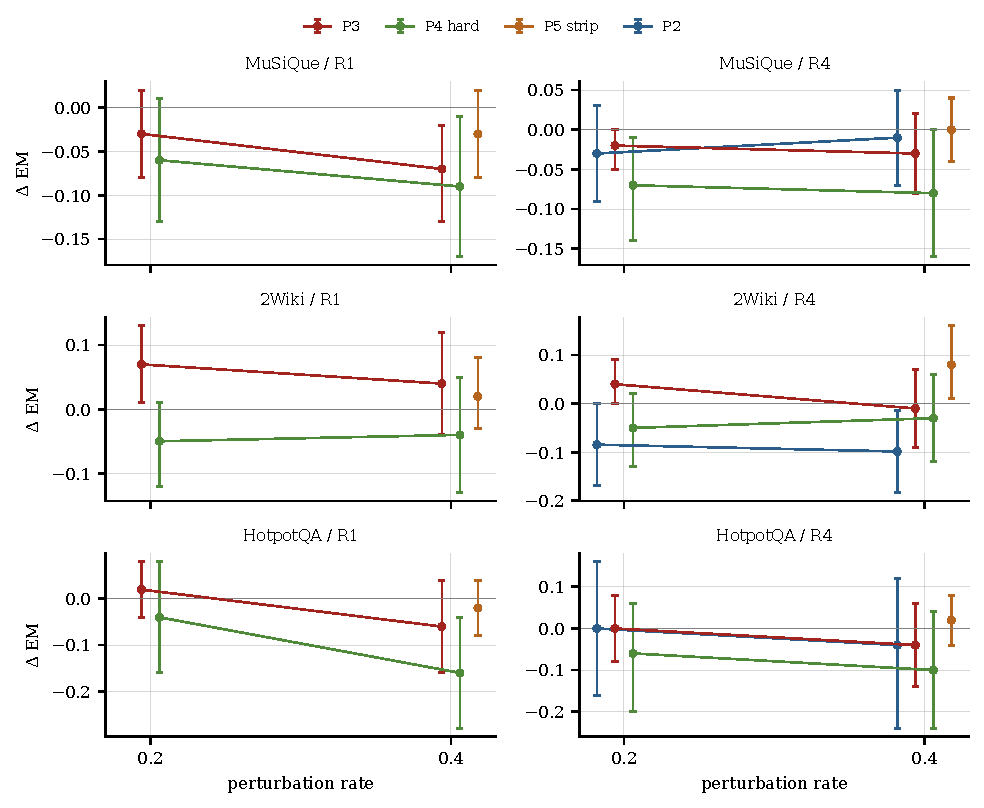
\includegraphics[width=0.8\textwidth]{figures/fig4_perturbation_sensitivity.pdf}
\caption{Exploratory pilot: change in exact match under label-preserving perturbations, relative to the same question unperturbed (95\% CIs). P1 and P6 can remove the answer and are reported in Table~\ref{tab:exp2} only.}
\label{fig:perturb}
\end{figure*}
\begin{figure*}[t]
\centering
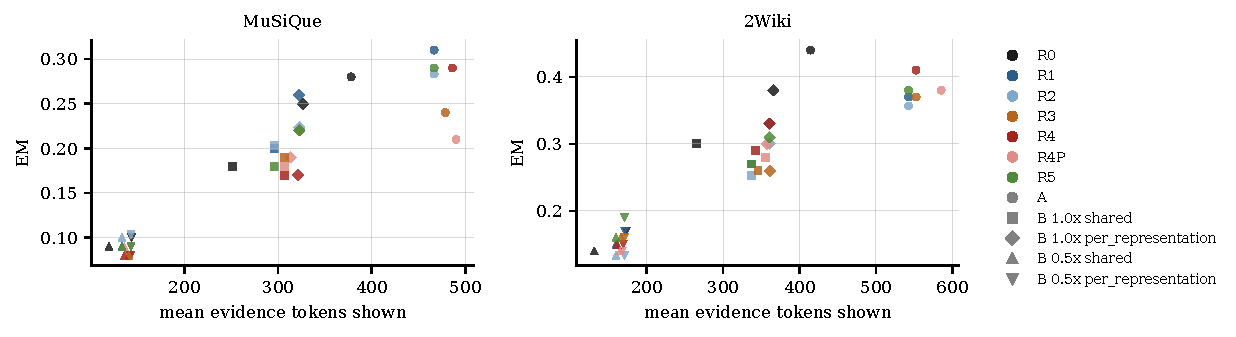
\includegraphics[width=0.85\textwidth]{figures/fig3_accuracy_vs_tokens.pdf}
\caption{Exploratory pilot: exact match against the mean number of evidence tokens shown, for Protocol~A (natural length) and Protocol~B (budget $1.0\times$ or $0.5\times$ the content tokens; shared or per-representation policy).}
\label{fig:budget}
\end{figure*}

\section{Revision experiments: supplementary tables}
\label{app:revision}

Table~\ref{tab:controls-strata} stratifies the contradiction-line effect by the number of such lines. Table~\ref{tab:contra-triage} summarises the predicted contradictions. Table~\ref{tab:retrieval} gives the retrieved-evidence contrasts under both protocols, and Table~\ref{tab:retrieval-strata} by retrieval outcome. Table~\ref{tab:exp0-costs} makes the budgets and costs of Experiment~0 explicit. All of these are exploratory. The blinded human-verification packages and their importers are described in the repository (\texttt{docs/REMAINING\_HUMAN\_VERIFICATION.md}).

\begin{table*}[t]
\centering
\footnotesize
\begin{adjustbox}{max width=\linewidth}
\begin{tabular}{@{}llrrrrlrrr@{}}
\toprule
Data & Change (second vs.\ first) & $n$ & $\Delta$EM & $\Delta$Abst. & $\Delta$Wrong & $\Delta$Acc.\ | both answered & C$\to$A / A$\to$C & C$\to$W / W$\to$C & W$\to$A / A$\to$W \\
\midrule
2Wiki & sentence items vs.\ passages & 3232 & -0.017 & +0.052 & -0.036 & +0.002 [-0.013, +0.017] & 87/29 & 152/156 & 163/52 \\
2Wiki & graph order vs.\ dataset order & 3232 & -0.008 & +0.012 & -0.004 & -0.006 [-0.018, +0.005] & 57/45 & 95/81 & 113/85 \\
2Wiki & derived relation lines vs.\ none & 3232 & +0.006 & +0.011 & -0.017 & +0.014 [+0.005, +0.024] & 42/29 & 42/74 & 81/59 \\
2Wiki & R4P vs.\ R4 (original) & 3232 & -0.036 & +0.061 & -0.025 & -0.017 [-0.027, -0.007] & 97/17 & 80/44 & 160/42 \\
2Wiki & contradiction lines on vs.\ off & 3232 & -0.033 & +0.061 & -0.028 & -0.013 [-0.022, -0.004] & 89/9 & 64/36 & 137/20 \\
\midrule
MuSiQue & sentence items vs.\ passages & 1744 & -0.001 & -0.009 & +0.010 & -0.004 [-0.020, +0.014] & 42/44 & 29/26 & 52/66 \\
MuSiQue & graph order vs.\ dataset order & 1744 & -0.011 & -0.003 & +0.015 & -0.025 [-0.045, -0.006] & 45/46 & 43/22 & 53/58 \\
MuSiQue & derived relation lines vs.\ none & 1744 & +0.010 & -0.004 & -0.006 & +0.013 [-0.007, +0.031] & 28/35 & 29/40 & 54/54 \\
MuSiQue & R4P vs.\ R4 (original) & 1744 & -0.045 & +0.089 & -0.044 & -0.012 [-0.037, +0.011] & 93/24 & 43/34 & 125/39 \\
MuSiQue & contradiction lines on vs.\ off & 1744 & -0.033 & +0.062 & -0.029 & -0.009 [-0.020, +0.003] & 52/2 & 14/7 & 64/6 \\
\bottomrule
\end{tabular}
\end{adjustbox}
\caption{Question-level outcome transitions (C correct, W answered and wrong, A not answered) between paired conditions on the confirmatory questions (exploratory decomposition). $\Delta$Acc.\ | both answered: accuracy difference among questions answered under both conditions, with 95\% CI. Sources: \texttt{revision/\allowbreak analysis/\allowbreak F\_exp1\_transitions.csv}, \texttt{revision/\allowbreak controls/\allowbreak controls\_transitions.csv}.}
\label{tab:transitions}
\end{table*}

\begin{figure*}[t]
\centering
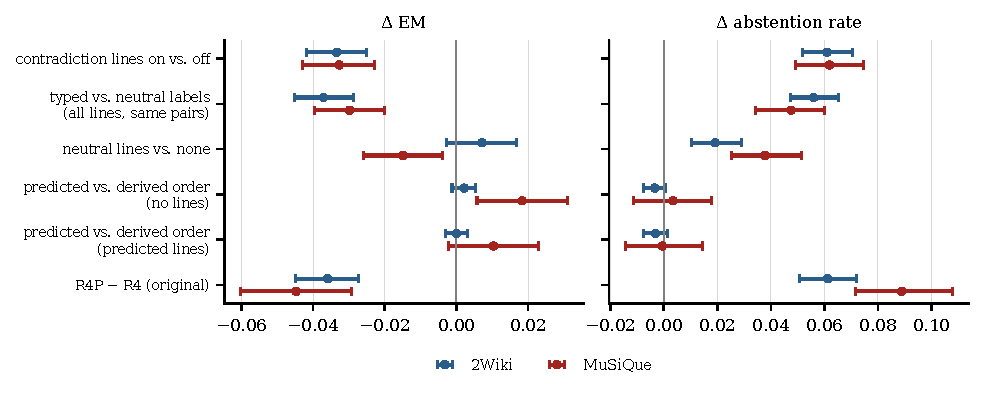
\includegraphics[width=0.9\textwidth]{figures/fig_controls.pdf}
\caption{Fixed-order relation controls on the confirmatory questions (exploratory). Each row changes one factor on identical facts; points are paired differences with 95\% CIs.}
\label{fig:controls}
\end{figure*}
\begin{table*}[t]
\centering
\footnotesize
\begin{adjustbox}{max width=\linewidth}
\begin{tabular}{@{}llrrlrl@{}}
\toprule
Data & Contradiction lines & $n$ & $\Delta$EM & 95\% CI & $\Delta$Abst. & 95\% CI \\
\midrule
2Wiki & 0 & 1198 & +0.000 & [+0.000, +0.000] & +0.000 & [+0.000, +0.000] \\
2Wiki & 1-2 & 1015 & -0.069 & [-0.089, -0.049] & +0.088 & [+0.068, +0.108] \\
2Wiki & 3-5 & 577 & -0.050 & [-0.075, -0.024] & +0.137 & [+0.106, +0.166] \\
2Wiki & 6+ & 442 & -0.020 & [-0.043, +0.002] & +0.066 & [+0.034, +0.097] \\
\midrule
MuSiQue & 0 & 734 & +0.000 & [+0.000, +0.000] & +0.000 & [+0.000, +0.000] \\
MuSiQue & 1-2 & 660 & -0.053 & [-0.073, -0.033] & +0.094 & [+0.071, +0.118] \\
MuSiQue & 3-5 & 257 & -0.039 & [-0.066, -0.016] & +0.132 & [+0.089, +0.179] \\
MuSiQue & 6+ & 93 & -0.129 & [-0.194, -0.065] & +0.129 & [+0.065, +0.204] \\
\bottomrule
\end{tabular}
\end{adjustbox}
\caption{Effect of showing the predicted \texttt{CONTRADICTS} lines (R4P\_FO$-$R4P\_FO\_NC) by the number of such lines in the prompt (exploratory). With no contradiction lines the two prompts are identical. Source: \texttt{revision/\allowbreak controls/\allowbreak relation\_control\_strata.csv}.}
\label{tab:controls-strata}
\end{table*}

\begin{table*}[t]
\centering
\footnotesize
\begin{adjustbox}{max width=\linewidth}
\begin{tabular}{@{}llrrlr@{}}
\toprule
Prompt & Contrast & $n$ & $\Delta$EM & 95\% CI & $\Delta$Abst. \\
\midrule
\texttt{qa-v2} & R1$-$R0 & 1000 & -0.023 & [-0.044, -0.002] & +0.059 \\
\texttt{qa-v2} & R4P$-$R4 & 1000 & -0.036 & [-0.054, -0.020] & +0.054 \\
\texttt{noabst} & R1$-$R0 & 1000 & -0.004 & [-0.026, +0.018] & +0.002 \\
\texttt{noabst} & R4P$-$R4 & 1000 & -0.017 & [-0.035, +0.000] & +0.003 \\
prompt effect & \texttt{noabst}$-$\texttt{qa-v2} (R0) & 1000 & +0.078 & [+0.055, +0.101] & -0.196 \\
prompt effect & \texttt{noabst}$-$\texttt{qa-v2} (R1) & 1000 & +0.097 & [+0.072, +0.123] & -0.253 \\
prompt effect & \texttt{noabst}$-$\texttt{qa-v2} (R4) & 1000 & +0.109 & [+0.084, +0.135] & -0.268 \\
prompt effect & \texttt{noabst}$-$\texttt{qa-v2} (R4P) & 1000 & +0.128 & [+0.103, +0.153] & -0.319 \\
interaction & (R1$-$R0) \texttt{noabst} minus \texttt{qa-v2} & 1000 & +0.019 & [-0.006, +0.045] & -0.057 \\
interaction & (R4P$-$R4) \texttt{noabst} minus \texttt{qa-v2} & 1000 & +0.019 & [-0.001, +0.040] & -0.051 \\
\bottomrule
\end{tabular}
\end{adjustbox}
\caption{Prompt factor (exploratory, 1{,}000 confirmatory 2Wiki questions): the frozen prompt \texttt{qa-v2} and the same prompt without the line offering \emph{insufficient evidence} (\texttt{noabst}); last rows give the prompt $\times$ representation interaction. Source: \texttt{revision/\allowbreak noabst/\allowbreak noabst\_contrasts.csv}.}
\label{tab:noabst}
\end{table*}

\begin{table*}[t]
\centering
\footnotesize
\begin{adjustbox}{max width=\linewidth}
\begin{tabular}{@{}lrr@{}}
\toprule
Automatic triage (heuristic, not a judgement) & Pairs & Share \\
\midrule
different source titles (different entities) & 3,857 & 40\% \\
same title, different years & 1,962 & 20\% \\
same title, different numbers & 671 & 7\% \\
same title, pronoun-initial sentence & 734 & 8\% \\
same title, other & 2,526 & 26\% \\
\midrule
all predicted contradiction pairs & 9,750 & 100\% \\
\bottomrule
\end{tabular}
\end{adjustbox}
\caption{Predicted \texttt{CONTRADICTS} pairs on the confirmatory sample (R4P; 12,816 directed edges, 12,372 rendered, 3,044 questions). NLI confidence $\geq$0.90 (median 0.985). Categories are heuristic triage for prioritising human verification. Source: \texttt{revision/\allowbreak contradictions/\allowbreak contradictions\_summary.json}.}
\label{tab:contra-triage}
\end{table*}

\begin{table*}[t]
\centering
\footnotesize
\begin{adjustbox}{max width=\linewidth}
\begin{tabular}{@{}lllrrrlrr@{}}
\toprule
Data & Prot. & Contrast & $n$ & Ident. & $\Delta$EM & 95\% CI & $\Delta$Abst. & Tokens \\
\midrule
MuSiQue & A & R1$-$R0 & 500 & 0 & +0.014 & [+0.000, +0.028] & -0.006 & 526$\to$653 \\
MuSiQue & A & R5$-$R1 & 500 & 451 & +0.010 & [+0.000, +0.020] & -0.008 & 653$\to$653 \\
MuSiQue & A & R4$-$R5 & 500 & 342 & +0.002 & [-0.012, +0.016] & -0.002 & 653$\to$657 \\
MuSiQue & A & R4P$-$R4 & 500 & 72 & -0.036 & [-0.056, -0.020] & +0.068 & 657$\to$701 \\
MuSiQue & A & contradiction lines on$-$off & 500 & 131 & -0.022 & [-0.038, -0.008] & +0.040 & 665$\to$701 \\
MuSiQue & A & R4P\_FO$-$R5 & 500 & 86 & -0.022 & [-0.038, -0.008] & +0.052 & 653$\to$701 \\
MuSiQue & B 1.0$\times$ & R1$-$R0 & 500 & 3 & +0.022 & [+0.002, +0.042] & +0.014 & 462$\to$457 \\
MuSiQue & B 1.0$\times$ & R5$-$R1 & 500 & 459 & +0.002 & [-0.004, +0.008] & -0.002 & 457$\to$457 \\
MuSiQue & B 1.0$\times$ & R4$-$R5 & 500 & 370 & +0.006 & [-0.004, +0.018] & -0.006 & 457$\to$457 \\
MuSiQue & B 1.0$\times$ & R4P$-$R4 & 500 & 133 & -0.032 & [-0.050, -0.016] & +0.052 & 457$\to$452 \\
MuSiQue & B 1.0$\times$ & contradiction lines on$-$off & 500 & 201 & -0.016 & [-0.028, -0.006] & +0.026 & 455$\to$452 \\
MuSiQue & B 1.0$\times$ & R4P\_FO$-$R5 & 500 & 144 & -0.020 & [-0.038, -0.004] & +0.038 & 457$\to$452 \\
\midrule
2Wiki & A & R1$-$R0 & 500 & 5 & -0.026 & [-0.054, +0.002] & +0.072 & 525$\to$681 \\
2Wiki & A & R5$-$R1 & 500 & 498 & +0.000 & [+0.000, +0.000] & +0.000 & 681$\to$681 \\
2Wiki & A & R4$-$R5 & 500 & 322 & +0.010 & [-0.008, +0.028] & -0.006 & 681$\to$685 \\
2Wiki & A & R4P$-$R4 & 500 & 84 & -0.030 & [-0.054, -0.008] & +0.066 & 685$\to$749 \\
2Wiki & A & contradiction lines on$-$off & 500 & 110 & -0.024 & [-0.046, -0.004] & +0.068 & 695$\to$749 \\
2Wiki & A & R4P\_FO$-$R5 & 500 & 66 & -0.016 & [-0.042, +0.010] & +0.052 & 681$\to$749 \\
2Wiki & B 1.0$\times$ & R1$-$R0 & 500 & 23 & +0.010 & [-0.016, +0.034] & +0.030 & 454$\to$451 \\
2Wiki & B 1.0$\times$ & R5$-$R1 & 500 & 499 & +0.000 & [+0.000, +0.000] & +0.000 & 451$\to$451 \\
2Wiki & B 1.0$\times$ & R4$-$R5 & 500 & 383 & -0.002 & [-0.014, +0.010] & +0.004 & 451$\to$451 \\
2Wiki & B 1.0$\times$ & R4P$-$R4 & 500 & 157 & -0.040 & [-0.060, -0.020] & +0.054 & 451$\to$447 \\
2Wiki & B 1.0$\times$ & contradiction lines on$-$off & 500 & 195 & -0.036 & [-0.054, -0.018] & +0.044 & 451$\to$447 \\
2Wiki & B 1.0$\times$ & R4P\_FO$-$R5 & 500 & 141 & -0.044 & [-0.066, -0.022] & +0.064 & 451$\to$447 \\
\bottomrule
\end{tabular}
\end{adjustbox}
\caption{Retrieved evidence (exploratory, fresh disjoint sample of 500 questions per dataset): every representation renders the same four reranked passages; R4/R5 use annotation-derived edges restricted to retrieved sentence pairs (oracle structure on real retrieval). Protocol B: budget $1.0\times$ content tokens, per-representation policy. Source: \texttt{revision/\allowbreak retrieval/\allowbreak retrieval\_contrasts.csv}.}
\label{tab:retrieval}
\end{table*}

\begin{table*}[t]
\centering
\footnotesize
\begin{adjustbox}{max width=\linewidth}
\begin{tabular}{@{}lllrrlr@{}}
\toprule
Data & Contrast & Stratum & $n$ & $\Delta$EM & 95\% CI & $\Delta$Abst. \\
\midrule
MuSiQue & R1$-$R0 & retrieval: complete & 149 & +0.034 & [-0.007, +0.074] & -0.034 \\
MuSiQue & R1$-$R0 & retrieval: partial & 311 & +0.006 & [-0.006, +0.019] & +0.010 \\
MuSiQue & R1$-$R0 & retrieval: none & 40 & +0.000 & [+0.000, +0.000] & -0.025 \\
MuSiQue & R1$-$R0 & distractor heavy: True & 328 & +0.006 & [+0.000, +0.015] & +0.012 \\
MuSiQue & R1$-$R0 & long evidence: True & 249 & +0.012 & [-0.008, +0.032] & -0.020 \\
MuSiQue & contradiction lines on$-$off & retrieval: complete & 149 & -0.047 & [-0.094, -0.007] & +0.047 \\
MuSiQue & contradiction lines on$-$off & retrieval: partial & 311 & -0.013 & [-0.026, -0.003] & +0.039 \\
MuSiQue & contradiction lines on$-$off & retrieval: none & 40 & +0.000 & [+0.000, +0.000] & +0.025 \\
MuSiQue & contradiction lines on$-$off & distractor heavy: True & 328 & -0.012 & [-0.024, -0.003] & +0.034 \\
MuSiQue & contradiction lines on$-$off & long evidence: True & 249 & -0.016 & [-0.040, +0.004] & +0.036 \\
\midrule
2Wiki & R1$-$R0 & retrieval: complete & 262 & -0.057 & [-0.099, -0.015] & +0.080 \\
2Wiki & R1$-$R0 & retrieval: partial & 238 & +0.008 & [-0.025, +0.042] & +0.063 \\
2Wiki & R1$-$R0 & distractor heavy: True & 119 & +0.008 & [+0.000, +0.025] & +0.067 \\
2Wiki & R1$-$R0 & long evidence: True & 250 & -0.036 & [-0.072, +0.000] & +0.060 \\
2Wiki & contradiction lines on$-$off & retrieval: complete & 262 & -0.019 & [-0.050, +0.011] & +0.069 \\
2Wiki & contradiction lines on$-$off & retrieval: partial & 238 & -0.029 & [-0.055, -0.008] & +0.067 \\
2Wiki & contradiction lines on$-$off & distractor heavy: True & 119 & -0.008 & [-0.025, +0.000] & +0.050 \\
2Wiki & contradiction lines on$-$off & long evidence: True & 250 & -0.012 & [-0.040, +0.016] & +0.072 \\
\bottomrule
\end{tabular}
\end{adjustbox}
\caption{Retrieved evidence, Protocol A, by retrospective retrieval outcome (gold labels used only to stratify). Exploratory; small strata have wide intervals. Source: \texttt{revision/\allowbreak retrieval/\allowbreak retrieval\_contrasts.csv}.}
\label{tab:retrieval-strata}
\end{table*}

\begin{table*}[t]
\centering
\footnotesize
\begin{adjustbox}{max width=\linewidth}
\begin{tabular}{@{}llrrrrrrrrr@{}}
\toprule
Data & Sys. & EM & Cov. & Tok. & Units & Gold-pass.\ rec. & Ans.\ in ev. & Extr.\ calls & Latency (s) & CONTRA share \\
\midrule
MuSiQue & B0 & 0.06 & 0.23 & 493 & 4.0 & 0.44 & 0.34 & 0.0 & 0.4 & -- \\
MuSiQue & B1 & 0.12 & 0.33 & 538 & 4.0 & 0.53 & 0.44 & 0.0 & 0.4 & -- \\
MuSiQue & B2 & 0.13 & 0.36 & 1390 & 57.1 & 0.53 & 0.44 & 15.3 & 24.3 & -- \\
MuSiQue & B3 & 0.15 & 0.38 & 1667 & 57.1 & 0.53 & 0.44 & 15.3 & 24.4 & -- \\
MuSiQue & B4 & 0.03 & 0.18 & 442 & 11.9 & 0.55 & 0.31 & 15.1 & 23.8 & 0.55 \\
\midrule
2Wiki & B0 & 0.23 & 0.54 & 506 & 4.0 & 0.76 & 0.69 & 0.0 & 0.4 & -- \\
2Wiki & B1 & 0.26 & 0.54 & 501 & 4.0 & 0.80 & 0.78 & 0.0 & 0.4 & -- \\
2Wiki & B2 & 0.24 & 0.48 & 1436 & 56.4 & 0.80 & 0.78 & 14.7 & 23.9 & -- \\
2Wiki & B3 & 0.20 & 0.50 & 1711 & 56.4 & 0.80 & 0.78 & 14.7 & 23.9 & -- \\
2Wiki & B4 & 0.11 & 0.25 & 489 & 11.9 & 0.80 & 0.56 & 14.7 & 23.8 & 0.62 \\
\bottomrule
\end{tabular}
\end{adjustbox}
\caption{Experiment~0 with budgets and costs made explicit (pilot, $n$=100 per dataset). Budgets are \emph{not} matched: B2/B3 show about three times the tokens of B0/B1; B4 selects at most 12 claims within 450 tokens. Latency includes LLM claim extraction (original-call latency for cached calls). CONTRA share: fraction of B4's predicted relations labelled \texttt{CONTRADICTS}. Source: \texttt{revision/\allowbreak analysis/\allowbreak C\_exp0\_costs.csv}.}
\label{tab:exp0-costs}
\end{table*}


\begin{figure*}[t]
\centering
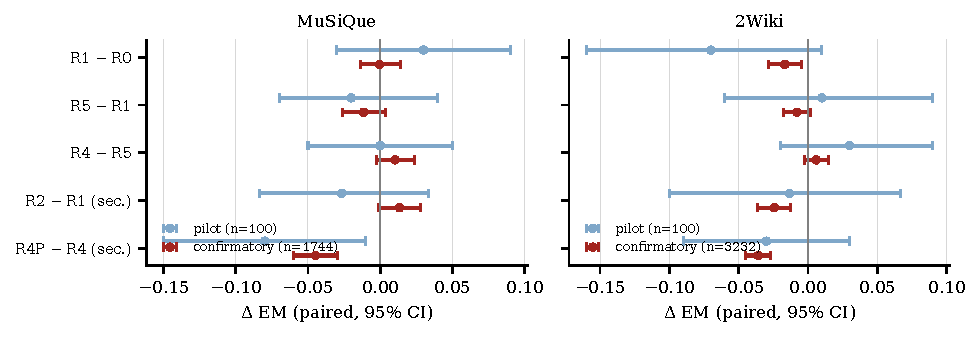
\includegraphics[width=0.85\textwidth]{figures/fig5_contrasts_pilot_vs_confirmatory.pdf}
\caption{Protocol~A contrasts in the exploratory pilot ($n$=100 per dataset) and on the disjoint confirmatory sample. The pilot estimate of R1$-$R0 on 2WikiMultiHopQA ($-0.07$) overstated the confirmed effect ($-0.017$) by a factor of four.}
\label{fig:forest}
\end{figure*}
